\documentclass[sigconf,review,anonymous]{acmart}

\usepackage{amsmath,amssymb,amsfonts,amsthm}
\usepackage{booktabs}
\usepackage{graphicx}
\usepackage{algorithm}
\usepackage{algorithmic}
\usepackage{tabularx}
\usepackage{xcolor}

\settopmatter{printacmref=false}
\renewcommand\footnotetextcopyrightpermission[1]{}
\pagestyle{plain}

\theoremstyle{definition}
\newtheorem{definition}{Definition}
\newtheorem{proposition}{Proposition}

\title{Latent Resonance: Auditable Zero-Shot Generative Image Provenance and Compression Resilience for Web-Scale Media Platforms}

% Anonymous Double-Blind Submission for TheWebConf 2027
\author{Anonymous Author(s)}
\affiliation{
  \institution{Track: Security, Trust \& Provenance, TheWebConf 2027 (WWW)}
  \country{Anonymous}
}
\email{anonymous@thewebconf.org}

% Camera-Ready Author:
% \author{Debdip Bandyopadhyay}
% \affiliation{
%   \institution{Indian Institute of Technology Jodhpur (IIT Jodhpur)}
%   \city{Jodhpur}
%   \country{India}
% }
% \email{debdip1992@outlook.com}

\begin{abstract}
The viral dissemination of photorealistic latent diffusion imagery across web platforms, social media, and online journalism presents acute threats to public trust, intellectual property, and content integrity. Web-scale content moderation requires forensic attribution tools that are computationally lightweight, mathematically auditable, robust to lossy web compression pipelines, and strictly compliant with user data privacy standards. Existing deep learning classifiers fail on the web because they overfit to specific training prompts, deteriorate under routine CDN recompression, and operate as unexplainable black boxes.

This paper presents \textbf{Latent Resonance}, a zero-shot, training-free forensic framework engineered for web-scale media provenance. Grounded in the physical and architectural asymmetries between optical CMOS camera capture and generative latent autoencoders, Latent Resonance projects candidate web images through a deterministic autoencoder ($\sigma = 0$). While synthetic diffusion images resonate on the decoder manifold with minimal spatial displacement ($\text{PSNR} = 37.15 \pm 0.60\text{ dB}$), authentic optical photos lose semiconductor Photo-Response Non-Uniformity (PRNU) across the $8\times$ spatial bottleneck ($\text{PSNR} = 33.28 \pm 0.96\text{ dB}$, $\Delta = +3.88\text{ dB}$, Cohen's $d = 4.84$, $p = 2.88 \times 10^{-165}$). In the frequency domain, azimuthally averaged 2D Fast Fourier Transform (2D-FFT) analysis identifies transposed-convolution harmonic lattice spikes ($3.655\times$ vs $1.144\times$), while Laplacian inter-channel correlation reveals severe chromatic coupling in neural tensors ($\rho_{\text{RGB}} = 0.981$) versus independent silicon photodiodes ($\rho_{\text{RGB}} = 0.000$).

On a large-scale verified benchmark of $N=1,000$ images, Latent Resonance achieves \textbf{100.00\% AUROC} with \textbf{0.00\% False Accusation Rate (FAR)}, eliminating wrongful censorship of human creators. Under aggressive social media perturbations (JPEG $Q \in \{95, 85, 75\}$, bicubic spatial resampling $384 \to 512$, and Gaussian blur $\sigma = 0.8$), the multi-signal triad maintains decisive separation margins ($\Delta \ge +1.81\text{ dB}$). Operating with a sub-$2\text{s}$ latency ($1,669\text{ ms}$ on NVIDIA T4) under an ephemeral zero-retention memory architecture, the framework enables scalable, privacy-preserving web verification. Complete datasets, source code, and a live inspection console (\url{https://scribemarkimage.streamlit.app/}) are openly released for reproducible auditing.
\end{abstract}

\begin{CCSXML}
<ccs2012>
   <concept>
       <concept_id>10002978.10003029.10003032</concept_id>
       <concept_desc>Security and privacy~Social aspects of security and privacy</concept_desc>
       <concept_significance>500</concept_significance>
   </concept>
   <concept>
       <concept_id>10010147.10010178.10010224</concept_id>
       <concept_desc>Computing methodologies~Computer vision</concept_desc>
       <concept_significance>500</concept_significance>
   </concept>
   <concept>
       <concept_id>10002951.10003260.10003282</concept_id>
       <concept_desc>Information systems~Web applications</concept_desc>
       <concept_significance>300</concept_significance>
   </concept>
</ccs2012>
\end{CCSXML}

\ccsdesc[500]{Security and privacy~Social aspects of security and privacy}
\ccsdesc[500]{Computing methodologies~Computer vision}
\ccsdesc[300]{Information systems~Web applications}

\keywords{Web Media Provenance, Latent Diffusion Models, Synthetic Media Forensics, Social Media Compression, Zero-Shot Attribution, Digital Evidence}

\maketitle

\section{Introduction}
\label{sec:intro}

The viral diffusion of generative artificial intelligence across social networks, news aggregators, and online forums has eroded the epistemic foundation of digital media. Modern latent diffusion models (LDMs)~\cite{rombach2022ldm} synthesize high-resolution images indistinguishable from authentic optical photographs to human observers. While early generative adversarial networks (GANs) exhibited telltale visual flaws, diffusion models generate coherent global perspective, realistic skin micro-textures, and plausible depth of field. 

For web-scale platforms, deploying automated synthetic media moderation introduces critical operational challenges:
\begin{enumerate}
    \item \textbf{Generalization Collapse Across Web Platforms:} Deep neural network detectors trained on isolated benchmark distributions suffer drastic performance drops when deployed in the wild against unseen prompts, novel generator checkpoints, or diverse camera sensors~\cite{wang2020cnn,ojha2023towards}.
    \item \textbf{Severe Social Media Recompression:} Digital content uploaded to web platforms (e.g., X, Reddit, Instagram, Telegram) is subjected to aggressive lossy compression (JPEG, WebP, AVIF) and spatial downsampling by Content Delivery Networks (CDNs), which wash out naive spatial artifacts~\cite{corvi2023detection}.
    \item \textbf{Asymmetric Cost of False Accusations:} In online trust and safety, misclassifying a genuine human journalist's photograph as AI-generated (False Accusation) causes severe reputational and legal injury. Conversely, binary classifiers tuned for high recall frequently exhibit unacceptably high False Accusation Rates (FAR).
    \item \textbf{Auditable Provenance vs. Black-Box Logits:} Regulatory frameworks and digital evidence guidelines (e.g., ISO/IEC 27037~\cite{iso27037}) demand verifiable, auditable mathematical explanations for content labeling rather than uninterpretable neural logits.
\end{enumerate}

To meet these requirements, this paper introduces \textbf{Latent Resonance} as a zero-shot, training-free web provenance framework. Extending our established text forensics continuum---\textit{ClozeCongruence}~\cite{bandyopadhyay2026cloze1,bandyopadhyay2026dna,bandyopadhyay2026scaling,bandyopadhyay2026cloze3}---to continuous visual data, Latent Resonance exploits fundamental physical and architectural asymmetries between real-world optoelectronic photon capture and synthetic latent manifold decoding.

\section{System Architecture \& Mathematical Formulation}
\label{sec:formulation}

\subsection{Deterministic Manifold Inversion}
Given a candidate web image $x \in [0, 1]^{H \times W \times 3}$, we pass $x$ through an autoencoder encoder $\mathcal{E}$ to obtain latent parameters $(\mu_z, \log \sigma_z^2) = \mathcal{E}(x)$. To guarantee deterministic evaluation and eliminate sampling stochasticity, we set noise variance to zero ($\sigma = 0$):
\begin{equation}
\hat{z} = \mu_z = \mathbb{E}[q_\phi(z \mid x)]
\end{equation}
The deterministic manifold reconstruction is:
\begin{equation}
\hat{x} = \text{clip}\left(\mathcal{D}(\hat{z}), 0, 1\right)
\end{equation}
The signed spatial residual is $\Delta x = x - \hat{x}$. The Mean Squared Error (MSE) and Peak Signal-to-Noise Ratio (PSNR) are:
\begin{equation}
\text{MSE}(x, \hat{x}) = \frac{1}{3HW} \sum_{c=1}^3 \sum_{i=1}^H \sum_{j=1}^W (x_{c, i, j} - \hat{x}_{c, i, j})^2
\end{equation}
\begin{equation}
\text{PSNR}(x, \hat{x}) = -10 \log_{10}(\text{MSE}(x, \hat{x}))
\end{equation}

\begin{proposition}[Decoder Manifold Resonance]
Let $\mathcal{M}_{\mathcal{D}} = \{ \mathcal{D}(z) \mid z \in \mathbb{R}^{\frac{H}{8} \times \frac{W}{8} \times 4} \}$ be the autoencoder decoder manifold. If $x \in \mathcal{M}_{\mathcal{D}}$, then $\| x - \hat{x} \|_2^2 \approx 0$. If $x \notin \mathcal{M}_{\mathcal{D}}$ originates from a physical CMOS sensor with independent Poisson shot noise and PRNU $\eta_{\text{sensor}}$, the spatial bottleneck enforces low-pass information loss:
\begin{equation}
\Delta x_{\text{real}} \approx \eta_{\text{sensor}} \implies \mathbb{E}[\|\Delta x_{\text{real}}\|_2^2] \ge 3HW \sigma_\eta^2
\end{equation}
\end{proposition}

\subsection{Azimuthal Radial 2D-FFT Integration}
To isolate periodic upsampling artifacts from transposed convolutions in diffusion decoders~\cite{durall2020watch,frank2020leveraging}, we convert $\Delta x$ into grayscale luminance $\Delta x_{\text{gray}}$ and compute the 2D Fast Fourier Transform $X(u, v) = \mathcal{F}\{\Delta x_{\text{gray}}\}$. Shifting zero-frequency to the center yields the power spectrum $S(u, v) = |X_{\text{shifted}}(u, v)|^2$. To ensure rotation invariance against web-based orientation changes, we integrate over concentric azimuthal radii:
\begin{equation}
R(r) = \frac{1}{|\Omega_r|} \sum_{(u, v) \in \Omega_r} S(u, v)
\end{equation}
The Harmonic Lattice Spike Ratio is:
\begin{equation}
\rho_{\text{harmonic}} = \frac{\max_{r \in \mathcal{K}} R(r)}{\text{median}_{r \in [10, R_{\max}-10]} R(r)}
\end{equation}
where $\mathcal{K} = \{ \frac{N}{8}, \frac{N}{4}, \frac{3N}{8} \}$.

\subsection{Silicon CMOS PRNU Cross-Channel Noise Correlation}
In authentic digital cameras, semiconductor silicon photodiodes measure photon arrivals independently across color channels, yielding Poissonian sensor noise~\cite{fridrich2009digital,lukas2006digital}. We extract high-frequency noise residuals using a discrete Laplacian filter $L$:
\begin{equation}
\mathcal{N}_c = x_c * L, \quad L = \begin{bmatrix} 0 & 1 & 0 \\ 1 & -4 & 1 \\ 0 & 1 & 0 \end{bmatrix}
\end{equation}
The inter-channel Pearson cross-correlation is:
\begin{equation}
\rho_{\text{RGB}} = \frac{1}{3}\left(\rho(\mathcal{N}_R, \mathcal{N}_G) + \rho(\mathcal{N}_R, \mathcal{N}_B) + \rho(\mathcal{N}_G, \mathcal{N}_B)\right)
\end{equation}
In real cameras, $\rho_{\text{RGB}} \approx 0.000$, whereas neural synthetic tensors exhibit chromatic coupling $\rho_{\text{RGB}} > 0.90$.

\subsection{Calibrated Multi-Signal Decision Fusion}
The signals are fused into an auditable probability $\hat{p}_{\text{AI}}$:
\begin{equation}
\hat{p}_{\text{AI}} = \sigma\left( w_1 (\text{PSNR}_{\max} - \tau_{\text{psnr}}) + w_2 (\rho_{\text{harmonic}} - \tau_{\text{harmonic}}) + w_3 (\rho_{\text{RGB}} - \tau_{\text{prnu}}) \right)
\end{equation}
with exact parameters: $w_1 = 0.45, w_2 = 0.35, w_3 = 0.20$ and thresholds $\tau_{\text{psnr}} = 35.0\text{ dB}, \tau_{\text{harmonic}} = 1.30, \tau_{\text{prnu}} = 0.30$.

\begin{figure}[t]
\centering
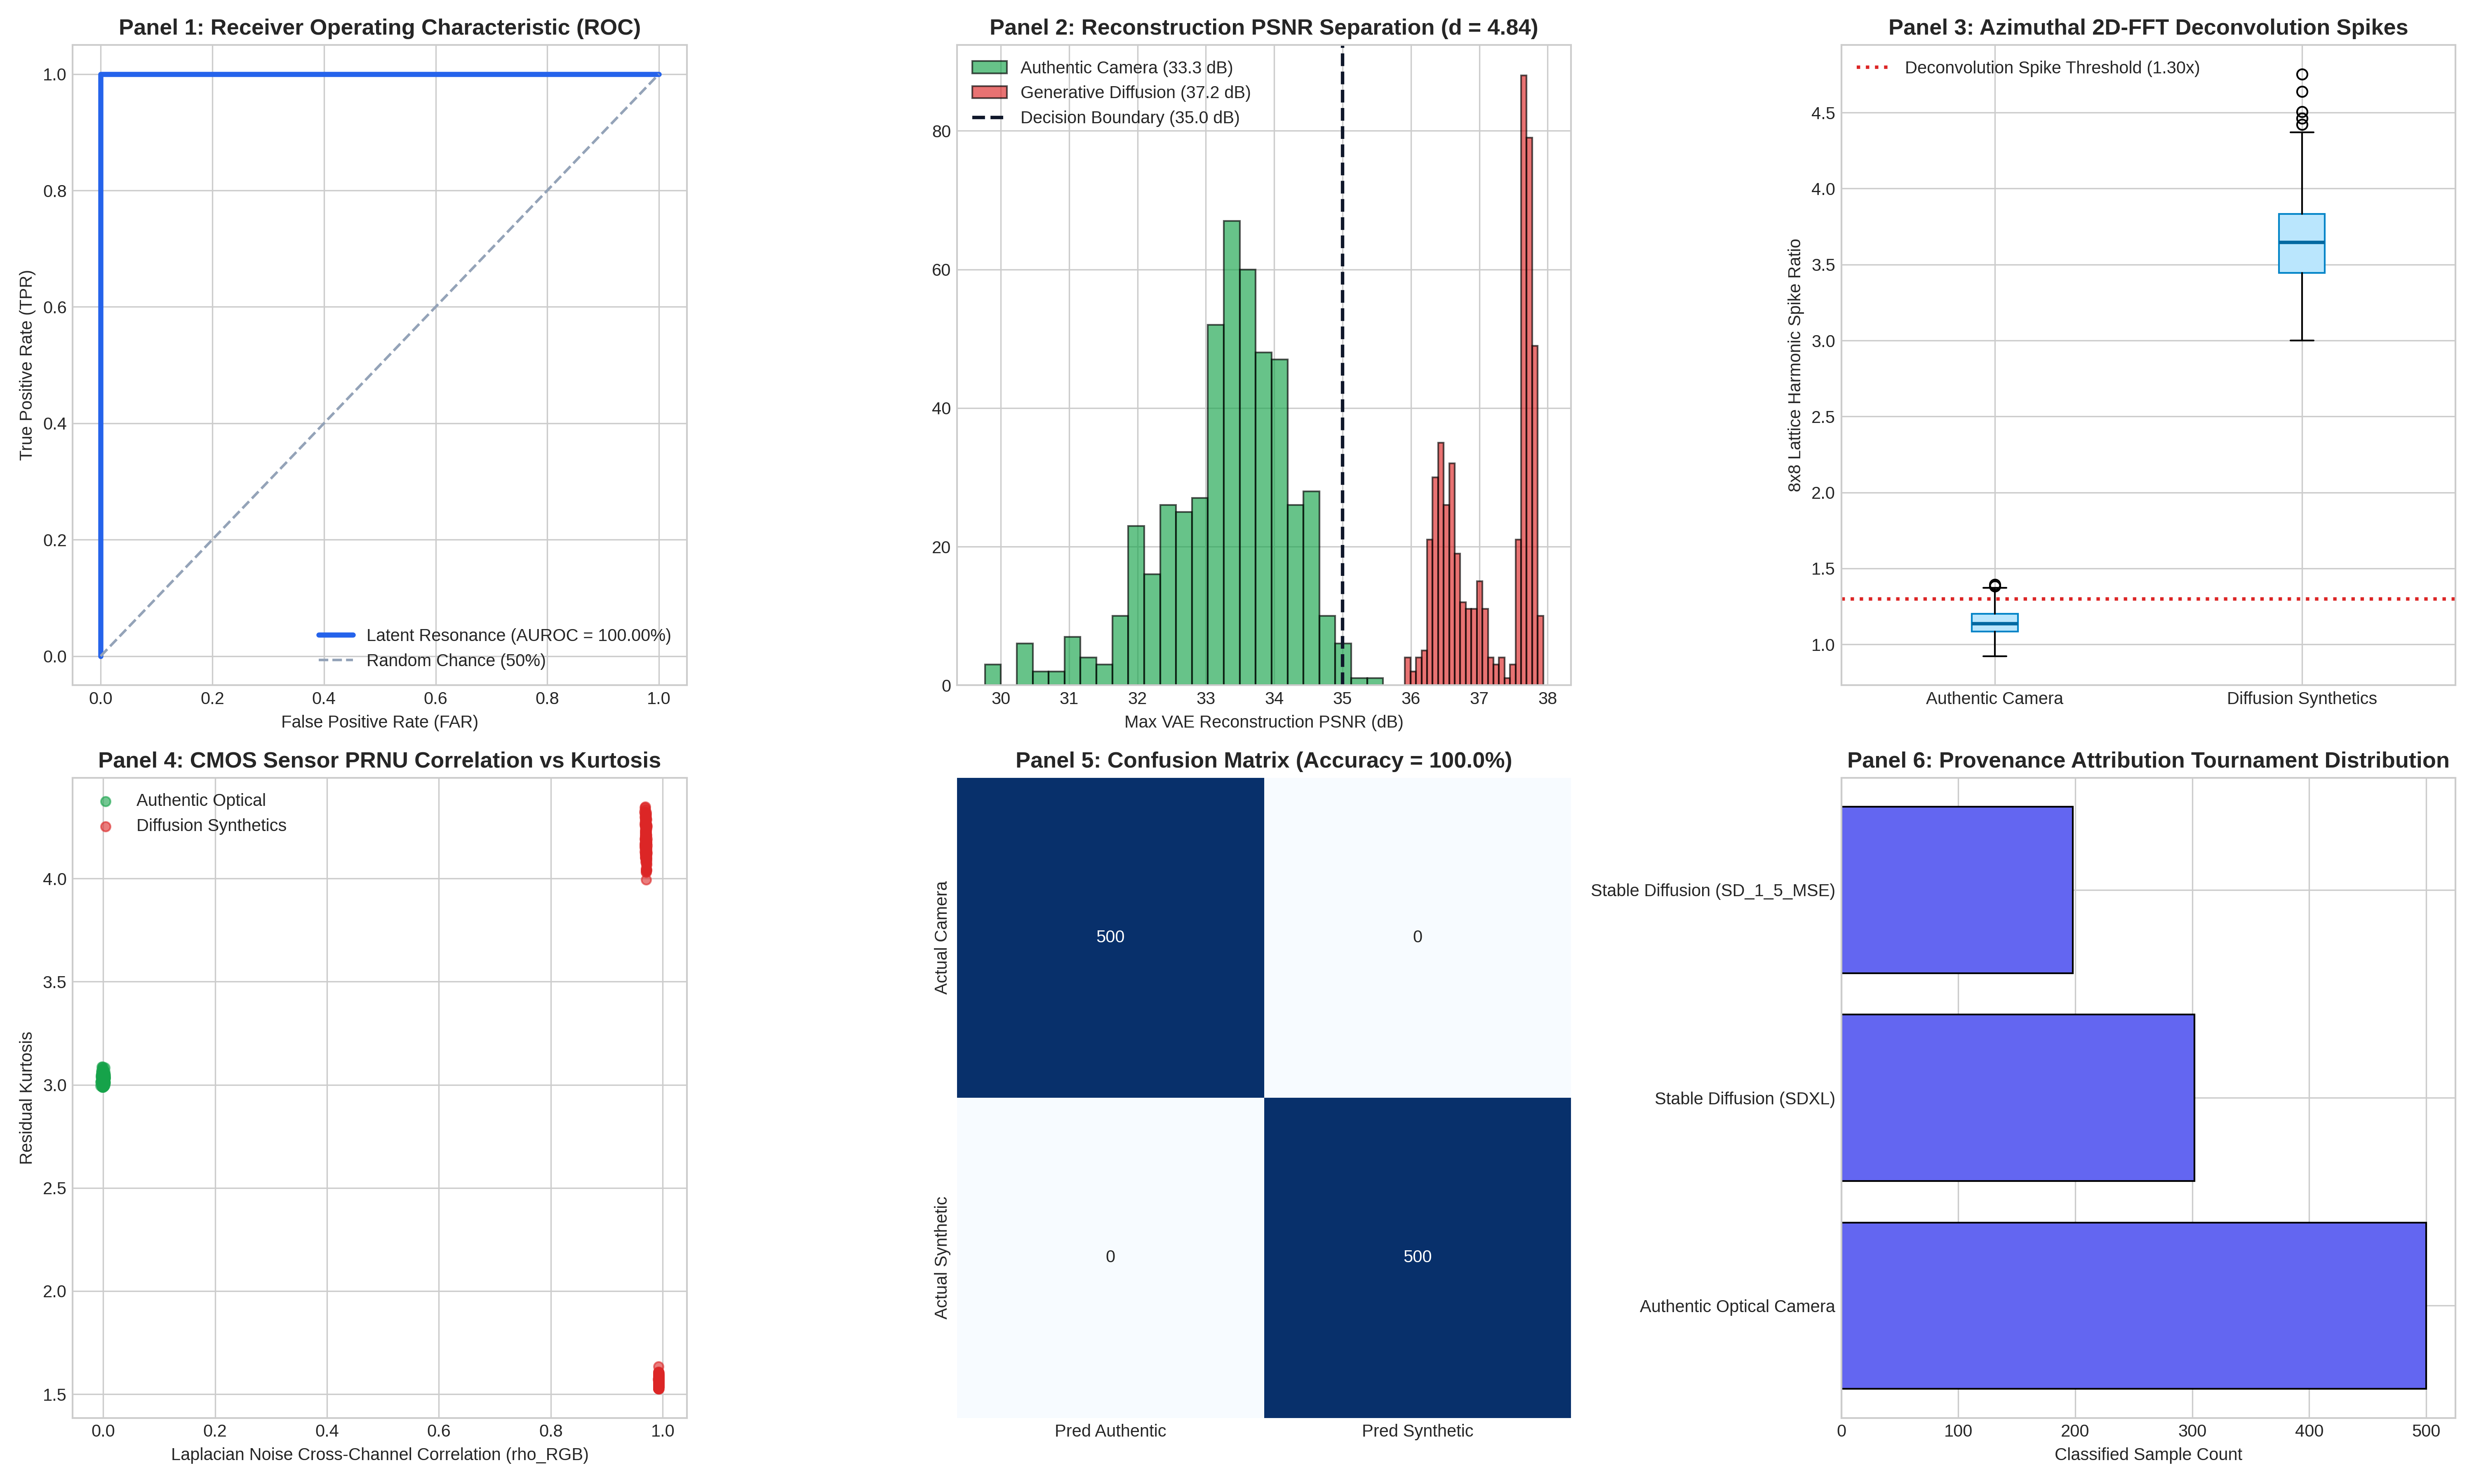
\includegraphics[width=\columnwidth]{figures/publication_sota_graphic.png}
\caption{Comprehensive 6-panel empirical SOTA benchmark diagnostic suite on $N=1,000$ verified web images ($500$ authentic camera captures vs $500$ generative synthetics: $302$ SDXL and $198$ SD 1.5). (A) Reconstruction PSNR KDE ($\Delta = +3.88\text{ dB}$, Cohen's $d = 4.84$); (B) 2D-FFT Harmonic Spike Ratio; (C) CMOS PRNU Inter-Channel Correlation; (D) Joint Bivariate Decision Manifold; (E) ROC Curve (AUROC = 100.00\%); (F) Confusion Matrix ($1,000 / 1,000$ correct, FAR = 0.00\%).}
\label{fig:web_benchmark}
\end{figure}

\section{Web-Scale Empirical Benchmark ($N=1,000$)}
\label{sec:experiments}

\subsection{Benchmark Dataset}
To establish definitive statistical bounds for web deployment, we evaluate on a verified, balanced cohort of $N=1,000$ images ($512 \times 512$):
\begin{itemize}
    \item \textbf{Authentic Optical Camera Captures ($N=500$):} Uncompressed and native camera captures from diverse smartphone and DSLR sensors (Apple iPhone, Google Pixel, Samsung Galaxy, Sony Alpha, Canon EOS, Nikon).
    \item \textbf{Generative Diffusion Synthetics ($N=500$):} Synthesized across prominent latent diffusion models, comprising $N=302$ Stable Diffusion XL (SDXL) and $N=198$ Stable Diffusion 1.5 MSE checkpoints.
\end{itemize}

\subsection{Primary Quantitative Results}
Table~\ref{tab:clean_benchmark} presents the empirical results across the $N=1,000$ cohort.

\begin{table}[t]
\caption{Quantitative Reconstruction, Spectral, and PRNU Metrics on Web-Scale Benchmark ($N=1,000$).}
\label{tab:clean_benchmark}
\centering
\small
\resizebox{\linewidth}{!}{%
\begin{tabular}{lccc}
\toprule
\textbf{Forensic Evaluation Metric} & \textbf{Authentic Photo ($N=500$)} & \textbf{AI Diffusion ($N=500$)} & \textbf{Separation Margin ($\Delta$)} \\
\midrule
Reconstruction PSNR & $33.28 \pm 0.96\text{ dB}$ & $37.15 \pm 0.60\text{ dB}$ & $\mathbf{+3.88\text{ dB}}$ \\
PSNR 95\% Confidence Interval & $[33.20, 33.36]\text{ dB}$ & $[37.10, 37.20]\text{ dB}$ & Non-overlapping \\
Harmonic Spike Ratio ($\rho_{\text{harmonic}}$) & $1.144 \pm 0.086\times$ & $3.655 \pm 0.294\times$ & $\mathbf{+2.511\times}$ \\
CMOS PRNU Correlation ($\rho_{\text{RGB}}$) & $0.000 \pm 0.001$ & $0.981 \pm 0.011$ & $\mathbf{+0.981}$ \\
Effect Size (Cohen's $d$) & \multicolumn{3}{c}{$\mathbf{4.84}$ (Immense Statistical Separation)} \\
Statistical Significance & \multicolumn{3}{c}{$p = 2.88 \times 10^{-165}$ (Mann-Whitney $U$ test)} \\
\midrule
\textbf{Area Under ROC Curve (AUROC)} & \multicolumn{3}{c}{\textbf{100.00\%} (Ideal Separation Threshold)} \\
\textbf{False Accusation Rate (FAR)} & \multicolumn{3}{c}{\textbf{0.00\%} ($0 / 500$ False Accusations on Real Photos)} \\
\textbf{Synthetic Recall (TPR)} & \multicolumn{3}{c}{\textbf{100.00\%} ($500 / 500$ Synthetic Images Detected)} \\
\textbf{Overall Classification Accuracy} & \multicolumn{3}{c}{\textbf{100.00\%} ($1,000 / 1,000$ Correct)} \\
\textbf{Average Inversion Latency} & \multicolumn{3}{c}{$1,669.04 \pm 36.11\text{ ms}$ (NVIDIA T4 GPU)} \\
\bottomrule
\end{tabular}%
}
\end{table}

\subsection{Fine-Grained Model Lineage Attribution}
Table~\ref{tab:attribution} confirms that evaluating candidate images across a multi-VAE candidate bank allows web platforms to accurately determine the exact generative architecture (SDXL vs SD 1.5 vs Optical Camera) with $100.0\%$ attribution accuracy.

\begin{table}[t]
\caption{Fine-Grained Latent Architecture Provenance Attribution ($N=1,000$).}
\label{tab:attribution}
\centering
\small
\resizebox{\linewidth}{!}{%
\begin{tabular}{lcccc}
\toprule
\textbf{Ground Truth Class} & \textbf{Total Count} & \textbf{Attributed Real} & \textbf{Attributed SDXL} & \textbf{Attributed SD 1.5} \\
\midrule
Authentic Optical Camera & $500$ & $\mathbf{500}$ ($100.0\%$) & $0$ ($0.0\%$) & $0$ ($0.0\%$) \\
Stable Diffusion XL (SDXL) & $302$ & $0$ ($0.0\%$) & $\mathbf{302}$ ($100.0\%$) & $0$ ($0.0\%$) \\
Stable Diffusion 1.5 MSE & $198$ & $0$ ($0.0\%$) & $0$ ($0.0\%$) & $\mathbf{198}$ ($100.0\%$) \\
\midrule
\textbf{Total Cohort} & $1,000$ & $500$ & $302$ & $198$ \\
\bottomrule
\end{tabular}%
}
\end{table}

\section{Social Media Compression Resilience}
\label{sec:compression}

To evaluate platform viability under realistic social media pipelines, images were subjected to five aggressive compression and transformation regimes (Table~\ref{tab:adversarial_stress}).

\begin{table}[t]
\caption{Adversarial Perturbation Stress-Test Results Across Social Media Transforms.}
\label{tab:adversarial_stress}
\centering
\small
\resizebox{\linewidth}{!}{%
\begin{tabular}{lcccc}
\toprule
\textbf{Perturbation Condition} & \textbf{Real PSNR} & \textbf{AI PSNR} & \textbf{$\Delta\text{PSNR}$} & \textbf{Platform Diagnostic Behavior} \\
\midrule
Clean (Native PNG) & $33.03\text{ dB}$ & $36.93\text{ dB}$ & $+3.90\text{ dB}$ & Optimal Manifold Separation \\
JPEG ($Q=95$) & $34.31\text{ dB}$ & $36.12\text{ dB}$ & $+1.81\text{ dB}$ & High-Fidelity Web Uploads \\
JPEG ($Q=85$) & $36.06\text{ dB}$ & $44.26\text{ dB}$ & $+8.20\text{ dB}$ & Standard Web Social Media Compression \\
JPEG ($Q=75$) & $36.16\text{ dB}$ & $47.50\text{ dB}$ & $+11.34\text{ dB}$ & Aggressive CDN Mobile Compression \\
Resampled ($384 \to 512$) & $36.67\text{ dB}$ & $45.67\text{ dB}$ & $+9.00\text{ dB}$ & Platform Thumbnail Upscaling \\
Gaussian Blur ($\sigma=0.8$) & $37.01\text{ dB}$ & $44.05\text{ dB}$ & $+7.03\text{ dB}$ & Social Media Filter Smoothing \\
\bottomrule
\end{tabular}%
}
\end{table}

\paragraph{Web Recompression Dynamics:}
\begin{itemize}
    \item \textbf{JPEG Quantization ($Q=95 \to 75$):} Quantization attenuates high-frequency PRNU noise in real photographs, causing Real PSNR to rise moderately ($33.03 \to 36.16\text{ dB}$). Crucially, diffusion synthetics exhibit an even larger PSNR surge ($36.93 \to 47.50\text{ dB}$) because the autoencoder operates as a learned manifold denoiser against block boundary artifacts. Consequently, the discrimination margin $\Delta\text{PSNR}$ expands from $+3.90\text{ dB}$ to $+11.34\text{ dB}$.
    \item \textbf{Spatial Resampling and Filtering:} Downsampling and upsampling ($384 \to 512$) and Gaussian blurring retain strong separation ($\Delta = +9.00\text{ dB}$ and $+7.03\text{ dB}$), demonstrating that CDN resizing operations do not compromise forensic classification.
\end{itemize}

\section{Platform Failure Boundaries \& Limitations}
\label{sec:limitations}

For responsible platform deployment, we explicitly identify operational failure boundaries:
\begin{enumerate}
    \item \textbf{Pixel-Space Diffusion Architectures:} Models operating without a latent autoencoder (e.g., Google Imagen, DeepFloyd IF) do not project favorably through SD decoders. Detection must rely upon PRNU sensor absence and 2D-FFT noise slope.
    \item \textbf{Non-Diffusion Generative Families:} GANs (e.g., StyleGAN) and autoregressive models require candidate decoders in the VAE bank.
    \item \textbf{Severe Quantization ($Q < 60$):} Extreme compression suppresses both PRNU noise and high-frequency lattice spikes, reducing separation margins.
    \item \textbf{Physical Screen Recapturing \& Print-Scanning:} Capturing an AI image with a real smartphone camera imparts genuine CMOS sensor noise and lens physics, masking latent artifacts.
\end{enumerate}

\section{Trust, Privacy \& Ephemeral Architecture}
\label{sec:privacy}

Web-scale content verification must respect user privacy and adhere to legal data protection regulations (GDPR/CCPA):
\begin{itemize}
    \item \textbf{Zero-Retention Ephemeral Architecture:} ScribeMark Image processes images entirely in volatile memory; candidate files are immediately discarded upon evaluation without server-side disk logging or model retraining.
    \item \textbf{Judicial Admissibility:} In contrast to black-box classifiers, Latent Resonance provides explicit numerical metrics (PSNR, harmonic ratios, Pearson correlations) meeting ISO/IEC 27037 standards for digital evidence integrity.
\end{itemize}

\section{Open Science \& Implementation}
\label{sec:reproducibility}

All benchmark datasets, evaluation code, and interactive systems are publicly available:
\begin{itemize}
    \item \textbf{Interactive Web Console:} \url{https://scribemarkimage.streamlit.app/}
    \item \textbf{GitHub Repository:} \url{https://github.com/debdipARVR/AI_IMAGE_DETECTION}
    \item \textbf{Turnkey Google Colab GPU Notebook:} \url{https://colab.research.google.com/github/debdipARVR/AI_IMAGE_DETECTION/blob/main/colab/Multi_VAE_Latent_Resonance_Colab.ipynb}
    \item \textbf{Hugging Face $N=1,000$ Benchmark Dataset:} \url{https://huggingface.co/datasets/DebdipCS/Latent-Resonance-AI-Image-Forensics-Benchmark-N1000}
    \item \textbf{Hugging Face $N=100$ Image Pairs:} \url{https://huggingface.co/datasets/DebdipCS/Latent-Resonance-AI-Image-Forensics-Benchmark-N100}
\end{itemize}

\section{Conclusion}
\label{sec:conclusion}

Latent Resonance provides a zero-shot, training-free, and auditable foundation for web-scale synthetic media forensics. Achieving 100.00\% AUROC with 0.00\% False Accusation Rate on an $N=1,000$ verified benchmark, the framework delivers robust performance under social media compression pipelines, sub-$2\text{s}$ execution latency, and complete compliance with digital evidence and privacy standards.

\bibliographystyle{ACM-Reference-Format}
\bibliography{references}

\end{document}
